\noindent
In this section, we first show through numerical simulations that the time to create the first sender, i.e., $T_1$, almost fully determines the overall broadcast time $T^*$. Next, we present an analytical treatment of the push technique for the minimum non-trivial case of $m=k=2$. In particular,  we attempt to compute the expected value of $T_1$ (i.e., $E(T_1)$) which is also supposed to provide an approximate estimation of $E(T^*)$. Finally, we provide pointers for the analytical treatment of the general $m=k$ case.  
We concentrate particularly on the complete graph topology; however, in a later subsection we also analytically study the message propagation for  
$m=k$ on infinite regular trees
\vspace{-3mm}
\subsection{Numerical simulations on complete graph topology}
\vspace{-1mm}



In this section, we give numeric evidence (with analytical support) that the
ratio of the overall broadcast time $T^{\ast }$ and the time to
create the first sender, i.e., $T_{1}$ converges for $n\rightarrow \infty$ to a constant which only depends on $k$. For this purpose we plot in figure~\ref%
{segSizeVsDelay_nrTrans_varyN_Mall_push_pull} the values of $Av(T^{\ast })$
and $Av(T_{1})$ respectively as we vary $n$ where $Av(x)$ represents the average of the quantity $x$ over several simulation runs. We report this distribution for
four different values of $m$ (2, 4, 8 and 16), in each case assuming that
there is only one message segment, i.e., $k=m$. Note that for B-P, the two quantities $Av(T^{\ast })$ and $Av(T_{1})$
exhibit a very similar profile irrespective of the value of $m$ chosen. In the same figure we also plot the function $n^{\frac{k-1}{k}}$ suitably scaled by a constant to show how the theoretical results which we provide in the following sections, closely approximate the numerical simulations. 

\begin{figure}[htbp] 
\centering
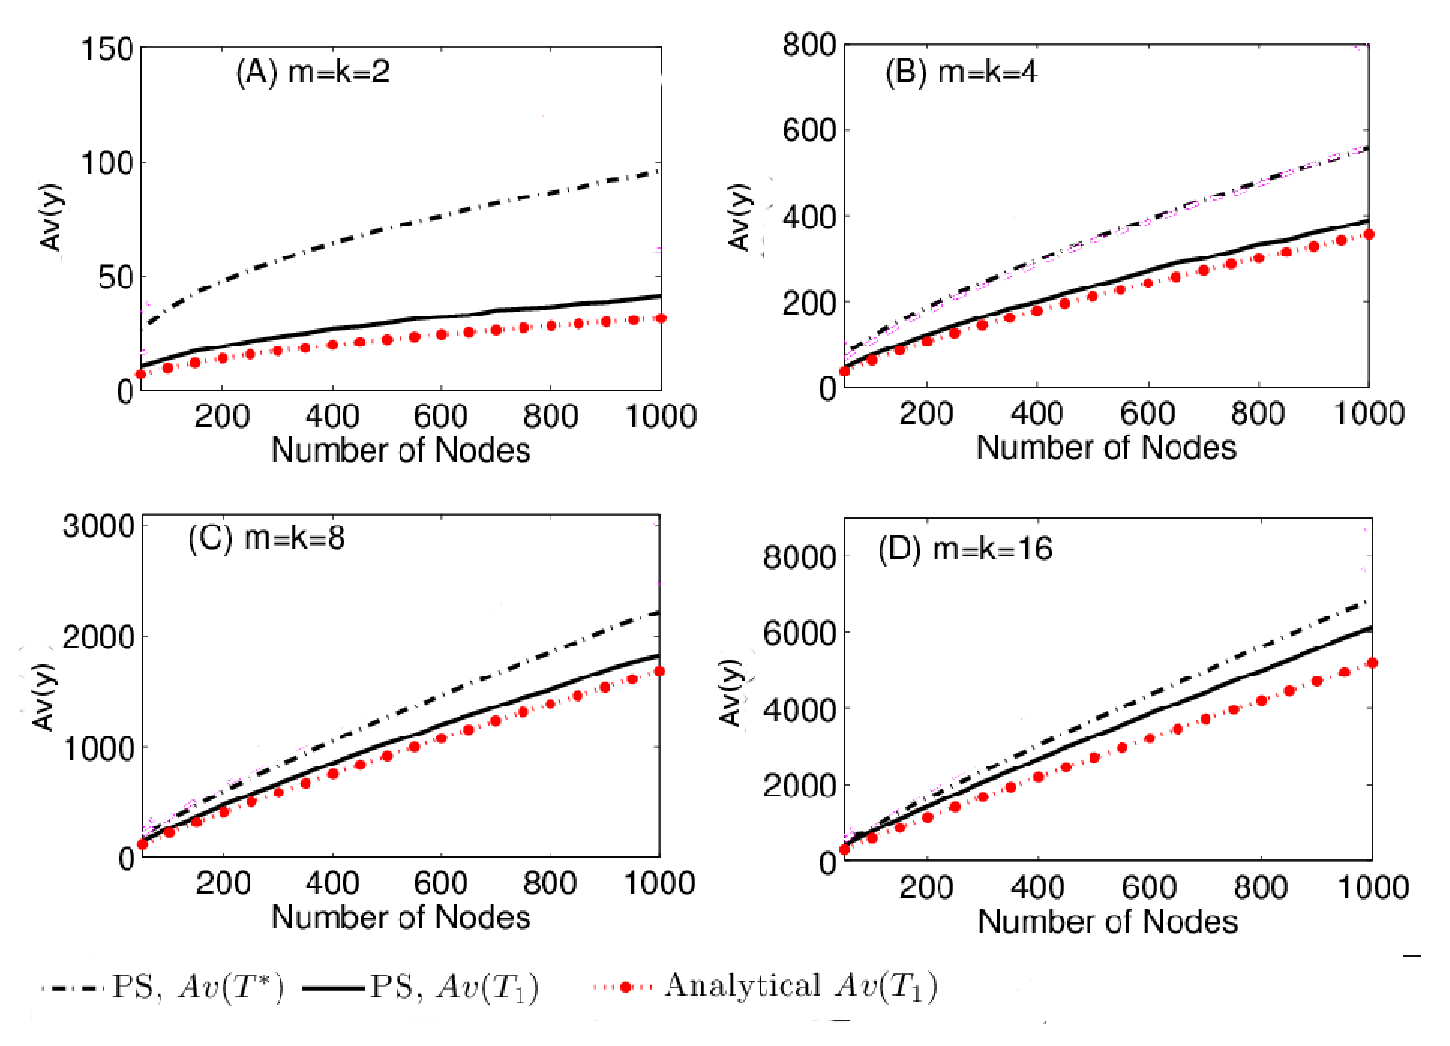
\includegraphics[scale=0.36]{figs1/segSizeVsDelay_nrTrans_varyN_Mall_push_pull2.eps}
\caption{$Av(T^*)$ and $Av(T_1)$ versus the number of nodes ($n$). Results are presented for (A) $m=k=2$, (B) $m=k=4$, (C) $m=k=8$, and (D) $m=k=16$. The plots also contain the suitably scaled function $n^{\frac{k-1}{k}}$ for each case.}
\label{segSizeVsDelay_nrTrans_varyN_Mall_push_pull}
\end{figure}
\vspace{-3mm}
\subsection{Performance of B-P in the limit $n\rightarrow \infty$ for complete graph topology}
\vspace{-1mm}


% We compute the expected time to obtain the first sender $E(T_{1})$ as well
% as the expected time $E\left( T^{\ast }\right) $ for broadcasting for a
% message which has $m=2$ packets ($p_{1}$ and $p_{2}$), and $s=1$ segment
% (i.e., the segment has $k=2$ packets). Recall that in push epidemic
% protocol, in each time step, a sender tries to establish a communication
% link with another agent. 
% %In each contact opportunity, only one packet can be
% %transferred from a sender to a receiver.
% As mentioned earlier, we assume only one packet can be transferred from a sender to a receiver in each contact opportunity. 
% 
% At the beginning, a source agent creates a message having 2 packets at time $%
% T_{0}$, this message has to be delivered to all other agents (i.e., $n-1$
% agents) in the network. The number of senders as a function of time is a
% step function and we denote the time of the $i^\textrm{th}$ step by $t_{i}.$ For $i$
% not too large  $\sum\limits_{j=1}^{i}t_{j}$ gives essentially the time $T_{i}$
% when the $i^\textrm{th}$ sender will be created, with the convention that $T_{0}=0$.
% Note that $\sum\limits_{i\geq 1}t_{i}$ is the broadcast time $T^{\ast }$ and 
% $t_{1}$ is the time when the first new sender is created.
% \vspace{-2mm}
% \begin{theorem}
% The random variable $\frac{t_{1}}{\sqrt{n}}$ converges as $n\rightarrow \infty $ to a
% limiting random variable $\tau _{1}$ with density $xe^{-\frac{x^{2}}{2}}$ and
% expectation $E\left( \tau _{1}\right) =\sqrt{\frac{\pi }{2}}.$ Furthermore
% for fixed $i\geq 2$ the random variable $\frac{t_{i}}{\sqrt{n}}$ converges to a
% limiting random variable $\tau _{i}$ and the following recursion holds for the
% expectations: $\frac{E\left( \tau _{i}\right) }{E\left( \tau _{i-1}\right) }%
% =\left( 1-\frac{3}{2i}\right) .$
% \end{theorem}
% \vspace{-2mm}
% \begin{theorem}
% $\frac{T^{\ast }}{\sqrt{n}}$ converges to a limiting random variable $s^{\ast }$ with $%
% E\left( s^{\ast }\right) =\sum\limits_{i=1}^{\infty }E\left( \tau
% _{i}\right) =2\cdot \sqrt{\frac{\pi }{2}}$
% \end{theorem}
% \vspace{-3mm}
% \begin{proof}
% (sketch). We will sketch in the following some of the important steps in the
% proof. For the probability that the first new sender is created at time $t$
% we have%
% \[
% \Pr \left\{ t_{1}=t\right\} =\frac{t-1}{n}\prod\limits_{l=1}^{t-2}\left( 1-%
% \frac{l}{n}\right) ,t\geq 2
% \]%
% Writing $\left( 1-\frac{l}{n}\right) =e^{-\frac{l}{n}+O\left( \frac{l^{2}}{%
% n^{2}}\right) }$we have for the cumulative distribution function 
% \begin{eqnarray*}
% \Pr \left\{ \frac{t_{1}}{\sqrt{n}}\leq x\right\}  &=&\sum\limits_{t\leq x%
% \sqrt{n}}\frac{t-1}{n}\prod\limits_{l=1}^{t-2}\left( 1-\frac{l}{n}\right)  \\
% &=&\sum\limits_{t\leq x\sqrt{n}}\frac{t}{n}e^{-\frac{t^{2}}{2n}+O\left( 
% \frac{t^{3}}{n^{2}}\right) }
% \end{eqnarray*}%
% For $n\rightarrow \infty $, the sum in the last expression converges to $%
% \int\limits_{0}^{x}ye^{-\frac{y^{2}}{2}}dy.$  Hence the limiting density is
% given by $ye^{-\frac{y^{2}}{2}}$ and the expectation by $\int\limits_{0}^{%
% \infty }y^{2}e^{-\frac{y^{2}}{2}}dy=\sqrt{\frac{\pi }{2}}.$ In a similar
% fashion one can obtain the conditional limiting distribution of $\tau _{i}$
% given the value of $b_{i-1}:=\sum\limits_{m=1}^{i-1}m\tau _{m}:$ 
% \[
% \Pr \left\{ \tau _{i}\leq x\right\} =\int\limits_{0}^{x}i\left(
% b_{i-1}+i\tau _{i}\right) e^{-i\left( \tau _{i}b_{i-1}+k\tau
% _{i}^{2}/2\right) }d\tau _{i}
% \]%
% Note that $b_{i}\sqrt{n}$ is the approximate number of nodes with one
% packet up to time $T_{i}.$ By a straightforward but lengthy computation
% using the previous expression for the conditional distribution of $\tau _{i}$
% it can be shown that the recursion $\frac{E\left( \tau _{i}\right) }{E\left(
% \tau _{i-1}\right) }=\left( 1-\frac{3}{2i}\right) $ holds. We will derive
% from this recursion now the expression for $s^{\ast }.$ Clearly we have 
% \[
% E\left( \tau _{i}\right) =\prod\limits_{j\geq 2}^{i}\frac{2j-3}{2j}E\left(
% \tau _{1}\right) 
% \]%
% and hence $s^{\ast }=\left( 1+\sum\limits_{i\geq 2}\prod\limits_{j\geq 2}^{i}%
% \frac{2j-3}{2j}\right) E\left( \tau _{1}\right) .$ Rewriting the product as%
% \[
% \prod\limits_{j\geq 2}^{i}\frac{2j-3}{2j}=\frac{\left( 2\left( i-1\right)
% \right) !}{4^{i-1}\left( \left( i-1\right) !\right) ^{2}i}
% \]%
% we have%
% \[
% s^{\ast }=\left( \sum\limits_{i=0}\frac{\left( 2i\right) !\cdot 2}{%
% 4^{i-1}\left( i!\right) ^{2}\cdot 2\left( i+1\right) }\right) E\left( \tau
% _{1}\right) 
% \]%
% The function 
% \[
% g\left( z\right) :=\sum\limits_{i=0}\frac{\left( 2i\right) !}{%
% 4^{i-1}\left( i!\right) ^{2}\cdot 2\left( i+1\right) }z^{2\left( i+1\right) }
% \]%
% converges for $\left\vert z\right\vert \leq 1$ and satisfies%
% \[
% \frac{d}{dz}g\left( z\right) =z\cdot \frac{d}{dz}\arcsin z=z\cdot \frac{1}{%
% \sqrt{1-z^{2}}}
% \]%
% as can be easily seen by comparing with the Taylor expansion of the right hand side. Hence 
% \[
% g\left( 1\right) =\int\limits_{0}^{1}\frac{z}{\sqrt{1-z^{2}}}dz=1
% \]%
% and $s^{\ast }=2E\left( \tau _{1}\right).$
% \end{proof}
% 
% It is important to note that the above computations can be carried out essentially up to a time $t$ where there are $\sqrt{n}$ senders. The remaining growth is very fast - actually of logarithmic order since several new senders in every time step get produced.
% \vspace{-3mm}
We compute the expected time to obtain the first sender $E(T_{1})$ as well
as the expected time $E\left( T^{\ast }\right) $ for broadcasting for a
message which has $m=2$ packets ($p_{1}$ and $p_{2}$), and $s=1$ segment
(i.e., the segment has $k=2$ packets). Recall that in push epidemic
protocol, in each time step, a sender tries to establish a communication
link with another agent. 
%In each contact opportunity, only one packet can be
%transferred from a sender to a receiver.
As mentioned earlier, we assume only one packet can be transferred from a
sender to a receiver in each contact opportunity.

At the beginning, a source agent creates a message having 2 packets at time $%
T_{0}$, this message has to be delivered to all other agents (i.e., $n-1$
agents) in the network. The number of senders as a function of time is a
step function and we denote the time of the $i^\textrm{th}$ step by $t_{i}.$
For $i$ not too large $\sum\limits_{j=1}^{i}t_{j}$ gives essentially the
time $T_{i}$ when the $i^\textrm{th}$ sender will be created, with the
convention that $T_{0}=0$. Note that $\sum\limits_{i\geq 1}t_{i}$ is the
broadcast time $T^{\ast }$ and $t_{1}$ is the time when the first new sender
is created. \vspace{-2mm} 
\begin{theorem}
The random variable $\frac{t_{1}}{\sqrt{n}}$ converges as $n\rightarrow \infty $ to a
limiting random variable $\tau _{1}$ with density $xe^{-\frac{x^{2}}{2}}$ and
expectation $E\left( \tau _{1}\right) =\sqrt{\frac{\pi }{2}}.$ Furthermore
for fixed $i\geq 2$ the random variable $\frac{t_{i}}{\sqrt{n}}$ converges to a
limiting random variable $\tau _{i}$ and the following recursion holds for the
expectations: $\frac{E\left( \tau _{i}\right) }{E\left( \tau _{i-1}\right) }%
=\left( 1-\frac{3}{2i}\right) .$
\end{theorem}
\vspace{-2mm} 
\begin{theorem}
$\frac{T^{\ast }}{\sqrt{n}}$ converges to a limiting random variable $s^{\ast }$ with $%
E\left( s^{\ast }\right) =\sum\limits_{i=1}^{\infty }E\left( \tau
_{i}\right) =2\cdot \sqrt{\frac{\pi }{2}}$
\end{theorem}
\vspace{-3mm} 
\begin{proof}
(sketch). We will sketch in the following some of the important steps in the
proof. For the probability that the first new sender is created at time $t$
we have%
\[
\Pr \left\{ t_{1}=t\right\} =\frac{t-1}{n}\prod\limits_{l=1}^{t-2}\left( 1-%
\frac{l}{n}\right) ,t\geq 2
\]%
Writing $\left( 1-\frac{l}{n}\right) =e^{-\frac{l}{n}+O\left( \frac{l^{2}}{%
n^{2}}\right) }$we have for the cumulative distribution function 
\begin{eqnarray*}
\Pr \left\{ \frac{t_{1}}{\sqrt{n}}\leq x\right\}  &=&\sum\limits_{t\leq x%
\sqrt{n}}\frac{t-1}{n}\prod\limits_{l=1}^{t-2}\left( 1-\frac{l}{n}\right)  \\
&=&\sum\limits_{t\leq x\sqrt{n}}\frac{t}{n}e^{-\frac{t^{2}}{2n}+O\left( 
\frac{t^{3}}{n^{2}}\right) }
\end{eqnarray*}%
For $n\rightarrow \infty $, the sum in the last expression converges to $%
\int\limits_{0}^{x}ye^{-\frac{y^{2}}{2}}dy.$  Hence the limiting density is
given by $ye^{-\frac{y^{2}}{2}}$ and the expectation by $\int\limits_{0}^{%
\infty }y^{2}e^{-\frac{y^{2}}{2}}dy=\sqrt{\frac{\pi }{2}}.$ In a similar
fashion one can obtain the conditional limiting distribution of $\tau _{i}$
given the value of $b_{i-1}:=\sum\limits_{m=1}^{i-1}m\tau _{m}:$ 
\[
\Pr \left\{ \tau _{i}\leq x\right\} =\int\limits_{0}^{x}i\left(
b_{i-1}+i\tau _{i}\right) e^{-i\left( \tau _{i}b_{i-1}+k\tau
_{i}^{2}/2\right) }d\tau _{i}
\]%
Note that $b_{i}\sqrt{n}$ is the approximate number of nodes with one
packet up to time $T_{i}.$ By a straightforward but lengthy computation
using the previous expression for the conditional distribution of $\tau _{i}$
it can be shown that the recursion $\frac{E\left( \tau _{i}\right) }{E\left(
\tau _{i-1}\right) }=\left( 1-\frac{3}{2i}\right) $ holds. We will derive
from this recursion now the expression for $s^{\ast }.$ Clearly we have 
\[
E\left( \tau _{i}\right) =\prod\limits_{j\geq 2}^{i}\frac{2j-3}{2j}E\left(
\tau _{1}\right) 
\]%
and hence $s^{\ast }=\left( 1+\sum\limits_{i\geq 2}\prod\limits_{j\geq 2}^{i}%
\frac{2j-3}{2j}\right) E\left( \tau _{1}\right) .$ Rewriting the product as%
\[
\prod\limits_{j\geq 2}^{i}\frac{2j-3}{2j}=\frac{\left( 2\left( i-1\right)
\right) !}{4^{i-1}\left( \left( i-1\right) !\right) ^{2}i}
\]%
we have%
\[
s^{\ast }=\left( \sum\limits_{i=0}\frac{\left( 2i\right) !\cdot 2}{%
4^{i-1}\left( i!\right) ^{2}\cdot 2\left( i+1\right) }\right) E\left( \tau
_{1}\right) 
\]%
The function 
\[
g\left( z\right) :=\sum\limits_{i=0}\frac{\left( 2i\right) !}{%
4^{i-1}\left( i!\right) ^{2}\cdot 2\left( i+1\right) }z^{2\left( i+1\right) }
\]%
converges for $\left\vert z\right\vert \leq 1$ and satisfies%
\[
\frac{d}{dz}g\left( z\right) =z\cdot \frac{d}{dz}\arcsin z=z\cdot \frac{1}{%
\sqrt{1-z^{2}}}
\]%
as can be easily seen by comparing with the Taylor expansion of the right hand side. Hence 
\[
g\left( 1\right) =\int\limits_{0}^{1}\frac{z}{\sqrt{1-z^{2}}}dz=1
\]%
and $s^{\ast }=2E\left( \tau _{1}\right).$
\end{proof}

It is important to note that the above computations can be carried out
essentially up to a time $t$ where there are $\sqrt{n}$ senders. The
remaining growth is very fast - actually of logarithmic order since several
new senders in every time step get produced. \vspace{-2mm}
\subsection{A short indication of the results for the general case $m=k$}
\vspace{-1mm}
% Here we present a sketch of the approach to general $m=k$ case. We are
% interested in the waiting time $t_{1}$ for the appearance of the first
% sender. For that, one has to understand how the number of sites which have
% exactly say $l$ packets grows with $t.$ 
% 
% (i) 1-packet carriers grow essentially as $t$ (because the initial sender
% node establishes contacts in most cases, a new node from the pool $n$),
% 
% (ii) 2-packet carriers grow essentially as $\sum\limits^{t}\frac{i}{n}\sim \frac{%
% t^{2}}{2n}$ since at time $i$ the probability to establish contact again from the $i$
% 1-packet carriers is $\frac{i}{n}.$~\footnote{This sum and all the
% following are random variables but for $t$ large enough one can use the
% central limit theorem -- furthermore the fluctuations are small compared to
% the leading term -- can all be worked out nicely and we plan to report this in a forthcoming paper.}
% 
% (iii) 3-packet carriers grow essentially as $\sum\limits^{t}\frac{1}{n}\frac{i^{2}%
% }{2n}\sim \frac{t^{3}}{3\cdot 2\cdot n^{2}}$,
% 
% \bigskip 
% 
% (iv) and finally the $(m-1)$-packet carriers grow essentially as $\frac{t^{m-1}}{\left(
% m-1\right) !n^{m-2}}$
% 
% With this estimation we can now proceed as in the $m=2$ case (conceptually of
% course) since%
% \begin{eqnarray*}
% \Pr \left( t_{1}=t\right)  &\sim &\frac{t^{m-1}}{\left( m-1\right) !n^{m-1}}%
% \prod\limits_{i}^{t}\left( 1-\frac{i^{m-1}}{\left( m-1\right) !n^{m-1}}%
% \right)  \\
% &\sim &\frac{t^{m-1}}{\left( m-1\right) !n^{m-1}}e^{-\frac{t^{m}}{m!n^{m-1}}}
% \end{eqnarray*}%
% From this one sees that $t_{1}$ is of the order $n^{\frac{m-1}{m}}$ .
% 
% More precisely one has for the limiting quantity $\tau
% _{1}=\lim_{n\rightarrow \infty }\frac{t_{1}}{n^{\frac{m-1}{m}}}:$%
% \[
% E\left( \tau _{1}\right) =\int\limits_{0}^{\infty }\frac{y^{m}}{\left(
% m-1\right) !}e^{-\frac{y^{m}}{m!}}dy
% \]%
% and $\tau _{1}$ has density $\frac{y^{m-1}}{\left( m-1\right) !}e^{-\frac{%
% y^{m}}{m!}}.$
Here we present a sketch of the approach to general $m=k$ case. We are
interested in the waiting time $t_{1}$ for the appearance of the first
sender. For that one has to understand how the number of sites which have
exactly say $l$ packets grows with $t.$

(i) 1-packet carriers grow essentially as $t$ (because the initial sender
node establishes contacts in most cases a new node from the pool $n$),

(ii) 2-packet carriers grow essentially as $\sum\limits^{t}\frac{i}{n}\sim 
\frac{t^{2}}{2n}$ since at time $i$ the probability to establish contact
again from the $i$ 1-packet carriers is $\frac{i}{n}.$~\footnote{%
This sum and all the following are random variables but for $t$ large enough
one can use the central limit theorem -- furthermore the fluctuations are
small compared to the leading term -- can all be worked out nicely and we
plan to report this in a forthcoming paper.}

(iii) 3-packet carriers grow essentially as $\sum\limits^{t}\frac{1}{n}\frac{%
i^{2}}{2n}\sim \frac{t^{3}}{3\cdot 2\cdot n^{2}}$,

\bigskip

(iv) and finally the $(m-1)$-packet carriers grow essentially as $\frac{%
t^{m-1}}{\left( m-1\right) !n^{m-2}}$

With this estimation we can now proceed as in the $m=2$ case (conceptually
of course) since%
\begin{eqnarray*}
\Pr \left( t_{1}=t\right) &\sim &\frac{t^{m-1}}{\left( m-1\right) !n^{m-1}}%
\prod\limits_{i}^{t}\left( 1-\frac{i^{m-1}}{\left( m-1\right) !n^{m-1}}%
\right) \\
&\sim &\frac{t^{m-1}}{\left( m-1\right) !n^{m-1}}e^{-\frac{t^{m}}{m!n^{m-1}}}
\end{eqnarray*}%
From this one sees that $t_{1}$ is of the order $n^{\frac{m-1}{m}}$ .

More precisely one has for the limiting quantity $\tau
_{1}=\lim_{n\rightarrow \infty }\frac{t_{1}}{n^{\frac{m-1}{m}}}:$%
\[
E\left( \tau _{1}\right) =\int\limits_{0}^{\infty }\frac{y^{m}}{\left(
m-1\right) !}e^{-\frac{y^{m}}{m!}}dy 
\]%
and $\tau _{1}$ has density $\frac{y^{m-1}}{\left( m-1\right) !}e^{-\frac{%
y^{m}}{m!}}.$

\subsection{Theoretical analysis for infinite regular trees}   
In this section we study the characteristics of message propagation with $m=k$ on
infinite regular trees. The same analysis provided here holds mutatis
mutandis for trees generated by branching processes with Poisson offspring
distribution.

We start with the case of $d$ $-$ regular trees for $d\geq 3$ with a
distinguished root index $0$ which acts as the initial sender. For
simplicity we give the root an out-degree of $d-1$ by attaching a virtual
``mother vertex'' to the root which is also a sender but has only one
offspring and is not counted in the estimation of sender nodes (this helps us avoid
handling the initial steps (when only the root is having the message)
differently from the later steps). Let $A_{l}\left( t\right) ,$ $0\leq l<m,$
be the number of nodes on the tree which have exactly $l$ packets at time $t
$ and have a direct communication link to one of the sender nodes at time $t$. Note that each of the so defined nodes has exactly one connection to a
sender node due to the tree structure and the initial condition of having
just one sender at the beginning. We get the following linear exact
recursion for the expectation $a_{l}\left( t+1\right) :=\mathbb{E}\left(
A_{l}\left( t+1\right) \right) $ at time $t+1:$%
\begin{eqnarray*}
a_{l}\left( t+1\right)  &=&\frac{k-1}{k}a_{l}\left( t\right) +\frac{1}{k}%
a_{l-1}\left( t\right) ,1\leq l\leq m-1 \\
a_{0}\left( t+1\right)  &=&\frac{k-1}{k}a_{m-1}\left( t\right) +\frac{k-1}{k}%
a_{0}\left( t\right) 
\end{eqnarray*}%
Note that for the expected number of sender nodes $s_{t}$ at time $t$ we
have 
\[
s_{t}=\sum\limits_{t^{\prime }<t}\frac{1}{k}a_{m-1}\left( t^{\prime }\right) 
\]
The asymptotic rate of growth of the variables $\left\{ a_{i}\left( t\right)
\right\} $ as well as $s_{t}$ is entirely determined by the value of the
largest eigenvalue of the associated transition matrix. The maximal
eigenvalue of the associated characteristic polynomial is given by 
\[
\lambda _{\max }=\frac{k-1}{k}+\left( \frac{k-1}{k}\left( \frac{1}{k}\right)
^{m-1}\right) ^{\frac{1}{m}}=\frac{k-1+\left( k-1\right) ^{1/m}}{k}
\]%
We study the maximum of the function $\frac{x-1+\left( x-1\right) ^{1/m}}{x}$
for $x>2.$ Setting the derivative to zero gives the condition 
\[
\left( x-1\right) ^{m-1}=\left( \frac{m-1}{m}x-1\right) ^{m},x>2
\]%
We therefore get
\[
\left( 1-\frac{x}{m\left( x-1\right) }\right) ^{m-1}\cdot \left( x-1-\frac{%
x}{m}\right)=1 
\]%
and in the limit $m\rightarrow \infty $ we obtain%
\[
\left( x-1\right) e^{-\frac{x}{x-1}}=1
\]%
Note that the whole computation holds also for the case of a Poisson
offspring distribution with expectation $k-1.$
\medskip